\section{Introduction}
Epilepsy is a neurological condition predominantly characterized by the protracted recurrence of
seizures. These temporary disturbances of neurological brain function affecting over 50 million
people worldwide have been attributed to various causes, such a stroke, head trauma, and infections.
However, patients may nonetheless present seizures of an unknown cause at the clinic, with resection
of epileptic tissue serves as a last line of defence. Therefore, further research must be conducted
to understand the mechanism through which epileptic seizures manifest for the future development of
targeted therapeutics. One avenue of research has focused on the SCNA1 gene, a sodium channel gene
with a history of mutations associated with epilepsy. For instance, mutants exhibit subtle
differences in voltage-gated sodium ion channel density along the cellular membrane. These changes
in channel density have been thought to underlie the physiological disturbance that results in
abnormal neurological functioning found in epilepsy. Here, we utilised two previously developed
models of SCNA1 mutations, the Q1489K and L1649Q variants, to gain a greater understanding of the
specific downstream cellular signalling mechanisms that are affected by changing the density of
mutated membrane sodium channels.

\section*{Methods - Signaling Model}
To investigate the impacts of sodium channel mutations on the downstream signalling dynamics within
the neuron, we considered two deterministic computational models. The first model uses a
Hodgkin-Huxley framework to determine the voltage and calcium readouts at various points in the
neuron (soma and dendrite) based on the various channel characteristics prescribed (Hay et al.).
Using this model, we stimulated the neuron at the soma and recorded voltage and calcium at the
dendrite for a control neuron and for neurons with various percentages of mutated sodium channels.
Based on the calcium readouts, we used the percent difference of the calcium peak between the
control case and mutated case as the input to the next model. The second model is a signalling model
of the signalling cascade following calcium influx into the neuron, based on Jedrzejewska-Szmek et
al. It should be noted that while Jedrzejewska-Szmek et al. used a multi-compartmental model, we use
a well-mixed model for simplicity. We modulate the calcium influx based on the results of model one,
and get GluR (AMPAR) as our readout.

\section{Results -- Signaling}
Using a combination of voltage and signaling models, we investigated the effects of sodium channel
mutations characteristic of epilepsy. We found that by changing the percentage of sodium channels
affected by this mutation, we can see departures from typical neuronal dynamics in regards to
voltage, calcium dynamics, and GluR levels. For the two SCNA1 mutations of interest, we see that
mutation 1 has a substantial jump in dendritic membrane voltage at 10\% mutation, while mutation 2
shows a jump at 15\% mutation, see Fig. \ref{volt}. Therefore, we will focus on mutation 1 for the
remainder of the analysis since lower percentages of its mutations can have a significant effect on
neuronal dynamics. We consider the maximum calcium concentration at the dendrite for mutation 1
trials and clearly see that maximum calcium concentration shows ultrasensitivity towards mutated
channel percentage. This switch-like behaviour occurs around 7.5\% mutation, see Fig. \ref{ultra}.
Therefore, once a neuron hits this threshold it will experience a significant increase in calcium.
We see that a similar trend is translated to GluR dynamics, see Fig. \ref{GluR}. We consider the
temporal dynamics of single phosphorylated GluR, and see that there is a similar jump between 5\%
and 10\% mutation. Initially GluR rises to a basal concentration, then at a critical time point
calcium dynamics begin to influence GluR. We see that the increase in 10-20\% mutation leads to
about twice the increase in GluR compared to the control and 5\% mutation. Therefore, we conclude
that at a critical level of mutated sodium channels, we get a increase in GluR levels which in turn
would cause feedback by affecting the neurons response to future action potentials and synaptic
communication.

\section{Discussion - Signaling}
The increased sensitivity of mutation 1 (Q1489K), in addition to the higher firing rates elicited by
increasing steps of current stimulation, reflect a gain-of-function relationship as the proportion
of mutated channels increases. This is in comparison to mutation 2 (L1649Q), which demonstrates the
opposite and appears to have a loss-of-function relationship as the proportion of mutated channels
increases. Interestingly, these relationship could be the opposite depending on the cellular
population affected. For example, epileptic seizures may be triggered by a loss of function of
inhibitory neurons, which may result in a gain of function of excitatory cortical neurons. Future
work should take into consideration the morphology of the modelled neurons, as their terminal
connections could affect their afferent networks differently depending on the multitude of terminal
synapses. In essence, a cortical neuron in a laminar structure may have limited spread of
overexcitation in comparison to a localized, inhibitory medium spiny neuron located in the striatum.
Another consideration is the location and nature of input stimulation. For example, our method could
be contrasted with simulated input from an upstream neuron, which may reflect the network in which a
neuron is situated more accurately. Furthermore, stimulation at the terminals could reveal the
voltage dynamics of our simulated mutant neurons in a way that would make their output to downstream
neurons measurable. For instance, stimulating at the dendrite of a mutant 1 (Q1489K) neuron could
reveal a greater voltage at the terminals, which may determine terminal output of vesicle release.


\begin{figure}[!!h]
    \centering
    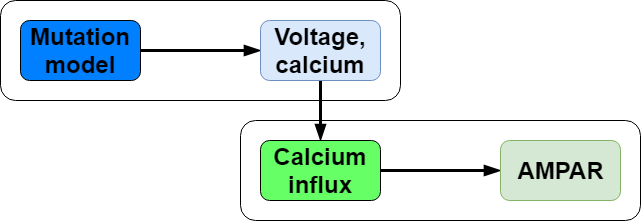
\includegraphics[width=\textwidth]{images/schematic.png}
    \caption{\textbf{Model Design} We combine two signaling models to investigate the impact of sodium channel mutations on calcium and AMPAR (GluR) dynamics.}
    \label{schematic}
\end{figure}

\begin{figure}[!!h]
    \centering
    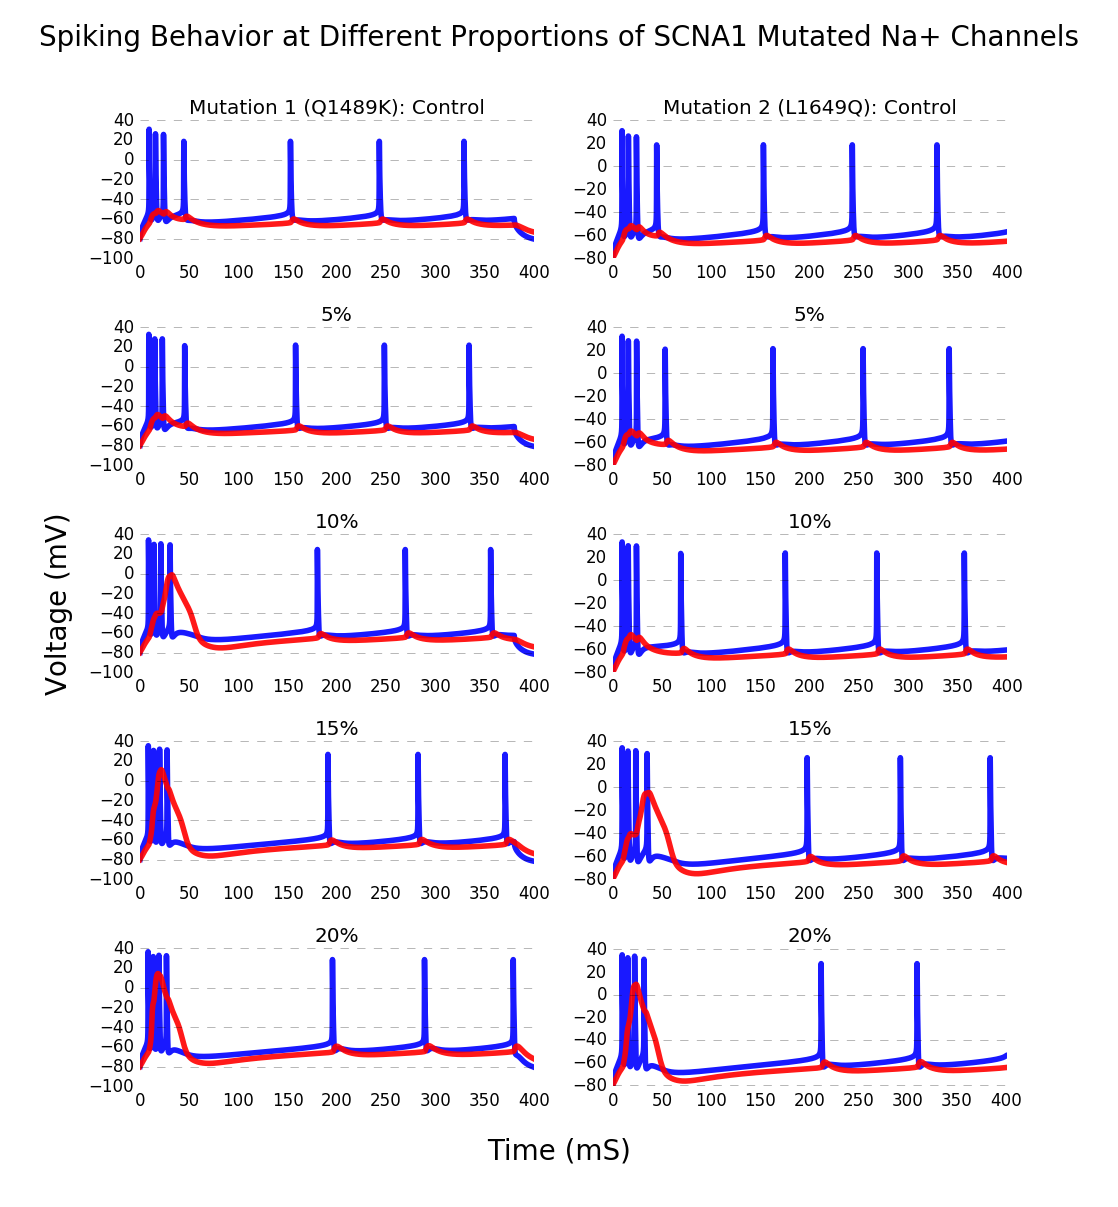
\includegraphics[width=1\textwidth]{images/spikes_all.png}
    \caption{\textbf{Voltage dynamics for two mutations} We model neurons with 0-20\% mutated sodium channels for two different types of mutations}
    \label{volt}
\end{figure}

\begin{figure}[!!h]
    \centering
    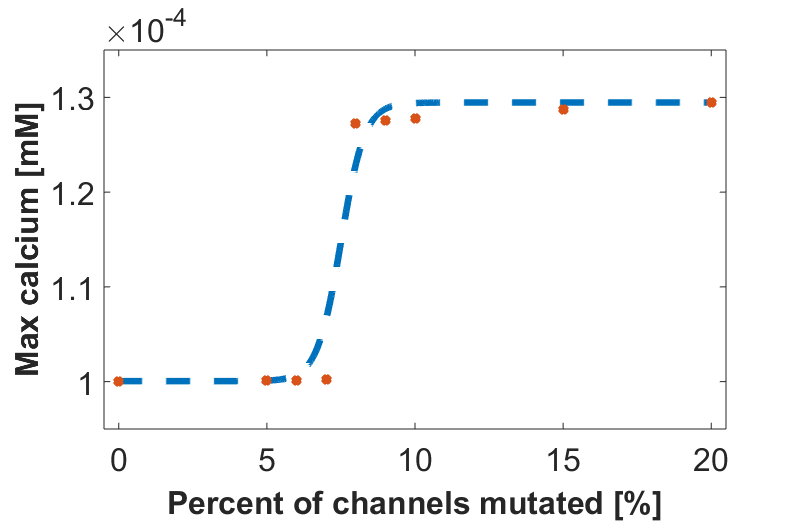
\includegraphics[width=1\textwidth]{images/ultraGraphSomaStim.png}
    \caption{\textbf{Calcium dynamics at the dendrite} We stimulated the neuron at the soma and recorded calcium readout at the dendrite. We found for mutation 1 that the calcium dependence of mutation percentage showed ultrasensitivity. For illustrative purposes, we have fit the data with a hyperbolic tangent to show the switch-like behavior around 7.5\% mutation.}
    \label{ultra}
\end{figure}

\begin{figure}[!!h]
    \centering
    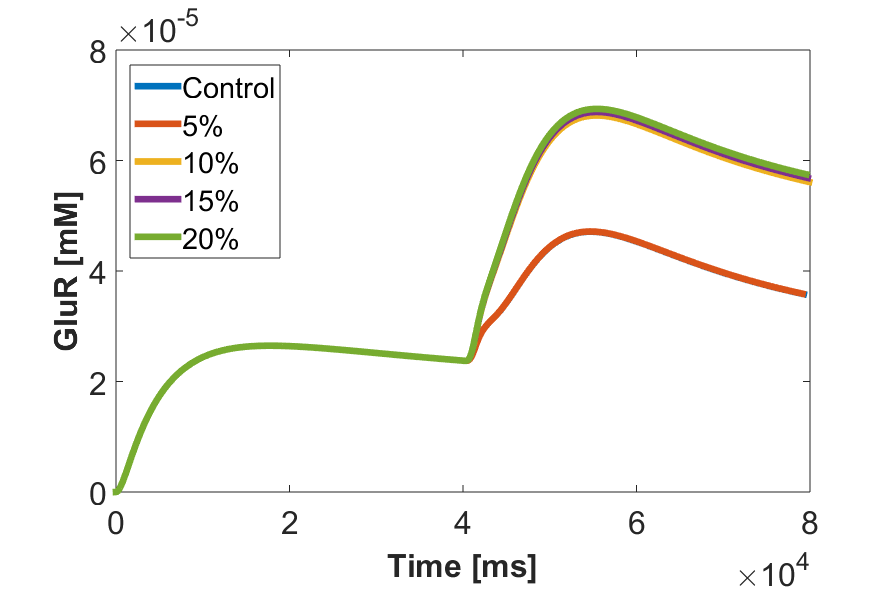
\includegraphics[width=1\textwidth]{images/GluRTimeSomaStim.png}
    \caption{\textbf{GluR dynamics} We modulate calcium influx into our signaling model based on the output of the voltage model to get our final readout of GluR. We see that all mutation levels show similar dynamics until a distinct time point in which 10\%, 15\%, and 20\% mutation all increase relative to the control.}
    \label{GluR}
\end{figure}
